\chapter[Processo de Desenvolvimento de Software]{Processo de Desenvolvimento de Software}
\label{cp:processo_de_desenvolvimento}

Como definido o tópico \ref{sec:processo_de_desenvolvimento_de_software}, foi elaborado um processo de desenvolvimento de \textit{software} deste projeto e que pode ser visualizado na Figura \ref{img:processo_de_desenvolvimento}.

\begin{figure}[H]
	\centering
	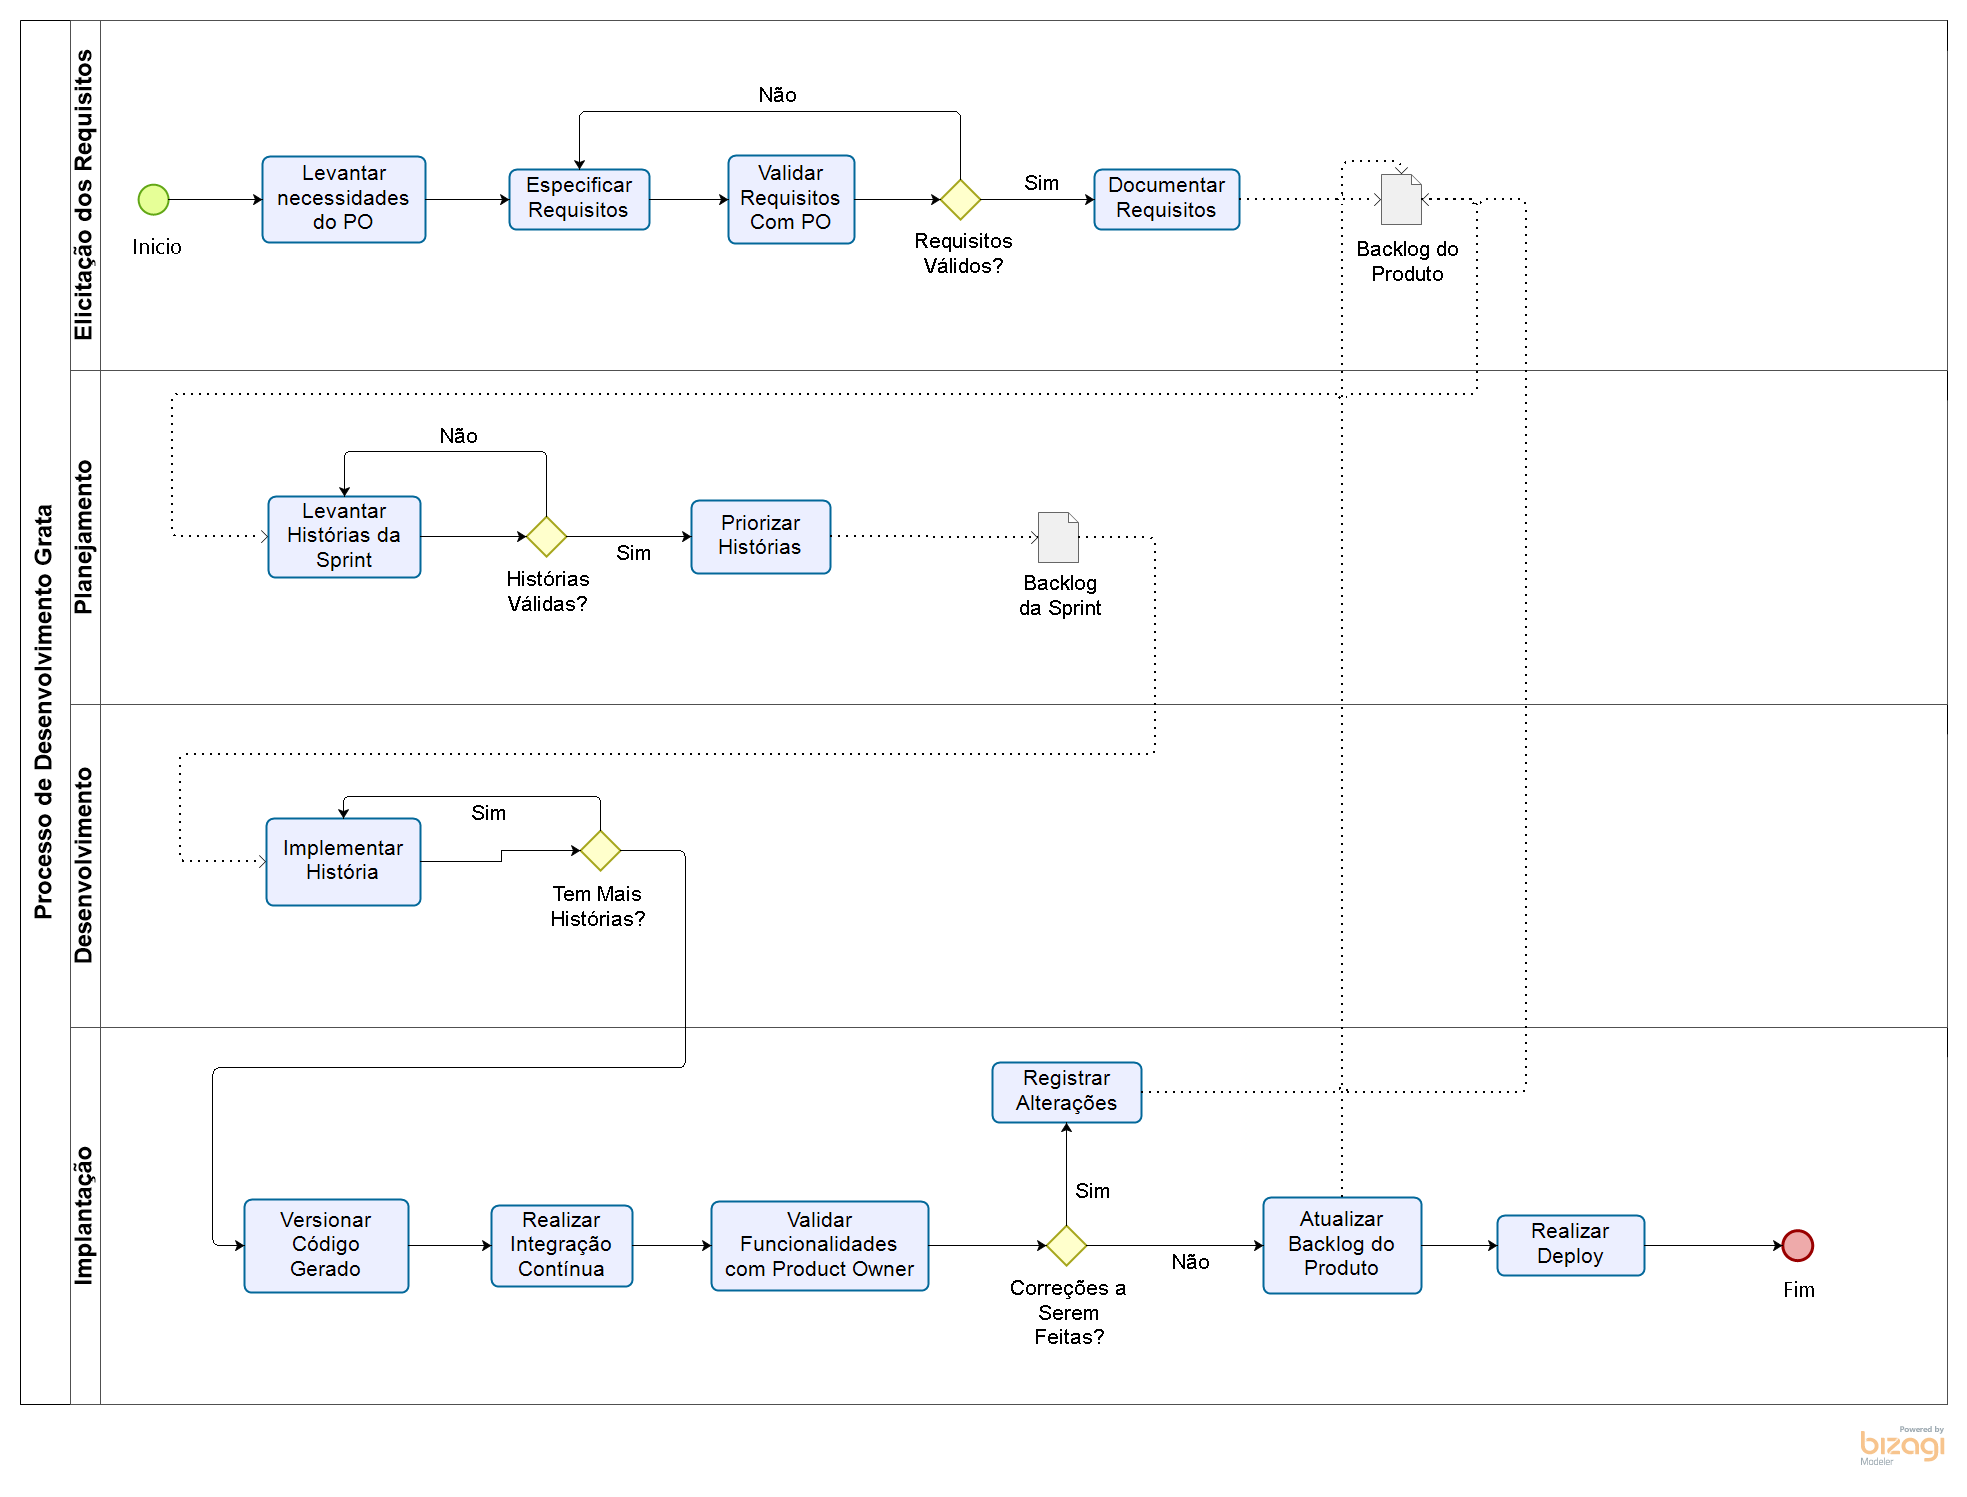
\includegraphics[width=1.0\textwidth]{figuras/processo_de_desenvolvimento.png}
	\caption{Processo de Desenvolvimento do Grata. Fonte: Própria}
	\label{img:processo_de_desenvolvimento}
\end{figure}

\section{Elicitação dos Requisitos}

De acordo com a Figura \ref{img:processo_de_desenvolvimento}, a primeira atividade a ser realizada é elicitação dos requisitos, definidos no tópico \ref{sec:elicitacao_requisitos}. As técnicas utilizadas para elicitação dos requisitos foram entrevista e observação, definidas respectivamente nos tópicos \ref{sec:entrevista} e \ref{sec:observacao}. 

A primeira atividade do processo \ref{img:processo_de_desenvolvimento} foi facilitada pois o desenvolvedor deste projeto estagia no setor do estudo de caso, NMIL, e com isso foram realizadas entrevistas a fim de entender como funciona todo o processo de marcar uma reunião até ela ser realizada. As entrevistas foram do tipo informal, pois assim foi possível entender melhor o contexto inserido. Esses processos podem ser visualizados nas Figuras \ref{img:modelagemProcessoGeral1Parte1}, \ref{img:modelagemProcessoGeral1Parte2}, \ref{img:modelagemProcessoGeral2Parte1} e \ref{img:modelagemProcessoGeral2Parte2}, que juntam englobam todo o processo do setor envolvendo reuniões, que conta com a presença de diversos participantes de diferentes setores.

Após realizar as entrevistas, foram realizadas observações sobre como os \textit{stakeholders} interagem com o sistema em vigor, e foi constatado que o sistema atual chamado Gertiq (Gerenciador de Tíquetes), ele é usado para marcar reuniões, contudo os participantes são chamados via email pela ferramenta \textit{Outlook}, não possuem um sistema para anotar as pautas e atas das reuniões, sendo feitas hoje a partir de folhas de papel.

\subsection{Requisitos Funcionais}

Para a elaboração dos requisitos funcionais, foi constatado a necessidade de uma identificação e descrição dos usuários do sistema, sendo apresentadas a seguir nas Tabelas \ref{tab:usuario_administrador} e \ref{tab:usuario_participante}: 

\begin{table}[H]
	\begin{tabular}{|p{3.0cm}|p{12.0cm}|} 
	\hline
	\textbf{Usuário} & \textbf{Administrador} \\ \hline
	\textbf{Descrição} & Usuário que irá ter total controle sobre o sistema e todas as funcionalidades.  \\ \hline
	\textbf{O que ele faz?} & Ele é responsável pela condução das reuniões, documentar as ATAs, apresentar relatórios e pauta das reuniões, acompanhar a evolução dos projetos, e receber \textit{feedbacks} sobre as reuniões. \\ \hline
	\textbf{O que ele precisa?} & Ele precisa de login e senha para conseguir acessar o sistema. visualizar um ambiente completo com todas as funcionalidades disponíveis no sistema. \\ \hline
	\end{tabular}
	 \caption{Usuário Administrador}
	 \label{tab:usuario_administrador}
\end{table}

\begin{table}[H]
	\begin{tabular}{|p{3.0cm}|p{12.0cm}|} 
	\hline
	\textbf{Usuário} & \textbf{Participante das Reunioes} \\ \hline
	\textbf{Descrição} & Usuário que irá acessar o sistema para visualizar a ATA das reuniões que participou. \\ \hline
	\textbf{O que ele faz?} & Contribui com informações nas reuniões usadas para gerar requisitos do produto. \\ \hline
	\textbf{O que ele precisa?} & Precisa de login e senha para conseguir acessar o sistema, visualizar as ATAas das reunioes que participou, podendo imprimir, baixar, e deixar comentários. \\ \hline
	\end{tabular}
	 \caption{Usuário Participante}
	 \label{tab:usuario_participante}
\end{table}

Após identificados e descritos os usuários do sistema, foi elaborado um diagrama de caso de uso, explicado no tópico \ref{sec:casos_de_uso}, sendo apresentado a seguir:

\begin{figure}[H]
	\centering
	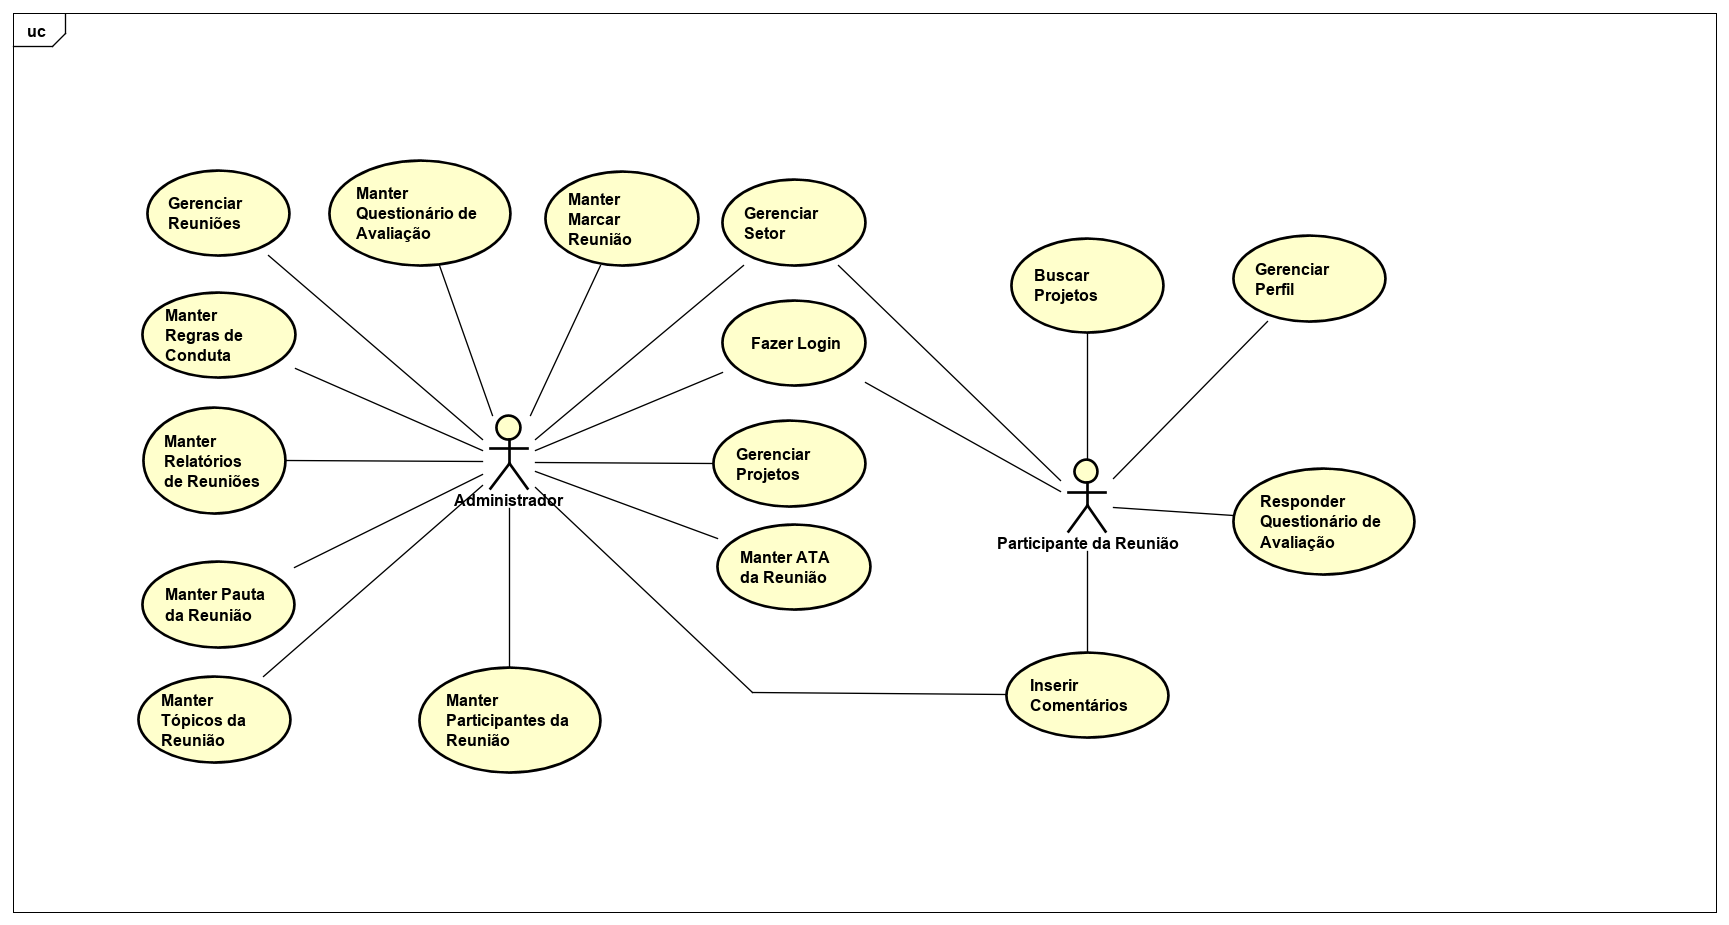
\includegraphics[width=1.0\textwidth]{figuras/casosDeUso.png}
	\caption{Casos de Uso Grata. Fonte: Própria}
	\label{img:casos_de_uso_grata}
\end{figure}

O diagrama de casos de uso da Figura \ref{img:casos_de_uso_grata} foi elaborado não apenas para visualização das funcionalidades, bem como as interações dos atores com o sistema, mas desenvolvido também como auxílio visual das funcionalidades para montar o \textit{backlog} do produto.

\subsubsection{Backlog do Produto}

O Backlog do Produto é composto pelas Histórias de Usuário e Histórias técnicas
elicitadas e desenvolvidas durante as Sprints. Estas representam necessidades levantadas reais para a aplicação, levantadas pelo PO e desenvolvedor.

\subsubsection{Histórias de Usuário}

As Histórias de Usuário representam as necessidades levantadas pelo usuário, que culminam em funcionalidades da aplicação. Nas Tabelas \ref{tab:historias_de_usuario_administrador_parte1}, \ref{tab:historias_de_usuario_administrador_parte2}, \ref{tab:historias_de_usuario_administrador_parte3}, e \ref{tab:historias_de_usuario_participante_parte1} são apresentadas as Histórias de Usuário elicitadas a partir da análise do diagrama de casos de uso da Figura \ref{img:casos_de_uso_grata}. 

\subsection{Requisitos Não-Funcionais}

Os requisitos não-funcionais, explicitados no tópico \ref{sec:requisitos_nao_funcionais}, são explicitados a seguir na Tabela \ref{tab:requisitos_nao_funcionais}:

\begin{table}[H]
	\begin{tabular}{|p{5.0cm}|p{10.0cm}|} 
	\hline
	\textbf{Requisito} & \textbf{Descrição} \\ \hline
	\textbf{Usabilidade} & O sistema de gerenciamento de reuniões e ATAs será construído para rodar em ambiente web. Deverá possuir um design responsivo. A interface do sistema deverá se comportar adequadamente independente do \textit{front-end} que será utilizado para o acesso - \textit{Browser, Smartphone} ou \textit{Tablet}. \\ \hline
	\textbf{Compatibilidade} & O sistema é desenvolvido para ser um sistema web, logo não deve apresentar problemas de compatibilidade entre \textit{browsers}, sendo eles o \textit{Google Chrome, Mozilla Firefox, Microsoft Edge e Safari}. \\ \hline
	\textbf{Segurança} & O sistema deve garantir a segurança dos dados mais críticos tais como senha dos usuários, cpf e \textit{emails}. \\ \hline
	\textbf{Validação} & O sistema deverá validar todos os campos obrigatórios tais como, nome do usuário, senha, nome e descrição da reunião. \\ \hline
	\textbf{Manutenção e Evolução} & O código deverá seguir padronização pela comunidade de \textit{software}, seguir recomendações de comentários em partes de código mais complexas, para assim facilitar a manutenção e evolução no futuro. \\ \hline
	\end{tabular}
	 \caption{Requisitos Não-Funcionais}
	 \label{tab:requisitos_nao_funcionais}
\end{table}

\subsection{Diagrama de Classe}

Para o desenvolvimento do sistema e auxiliar uma manutenção e evolução do sistema, foi montado um diagrama de classe que pode ser visto na Figura \ref{img:diagrama_de_classe}:

\begin{figure}[H]
	\centering
	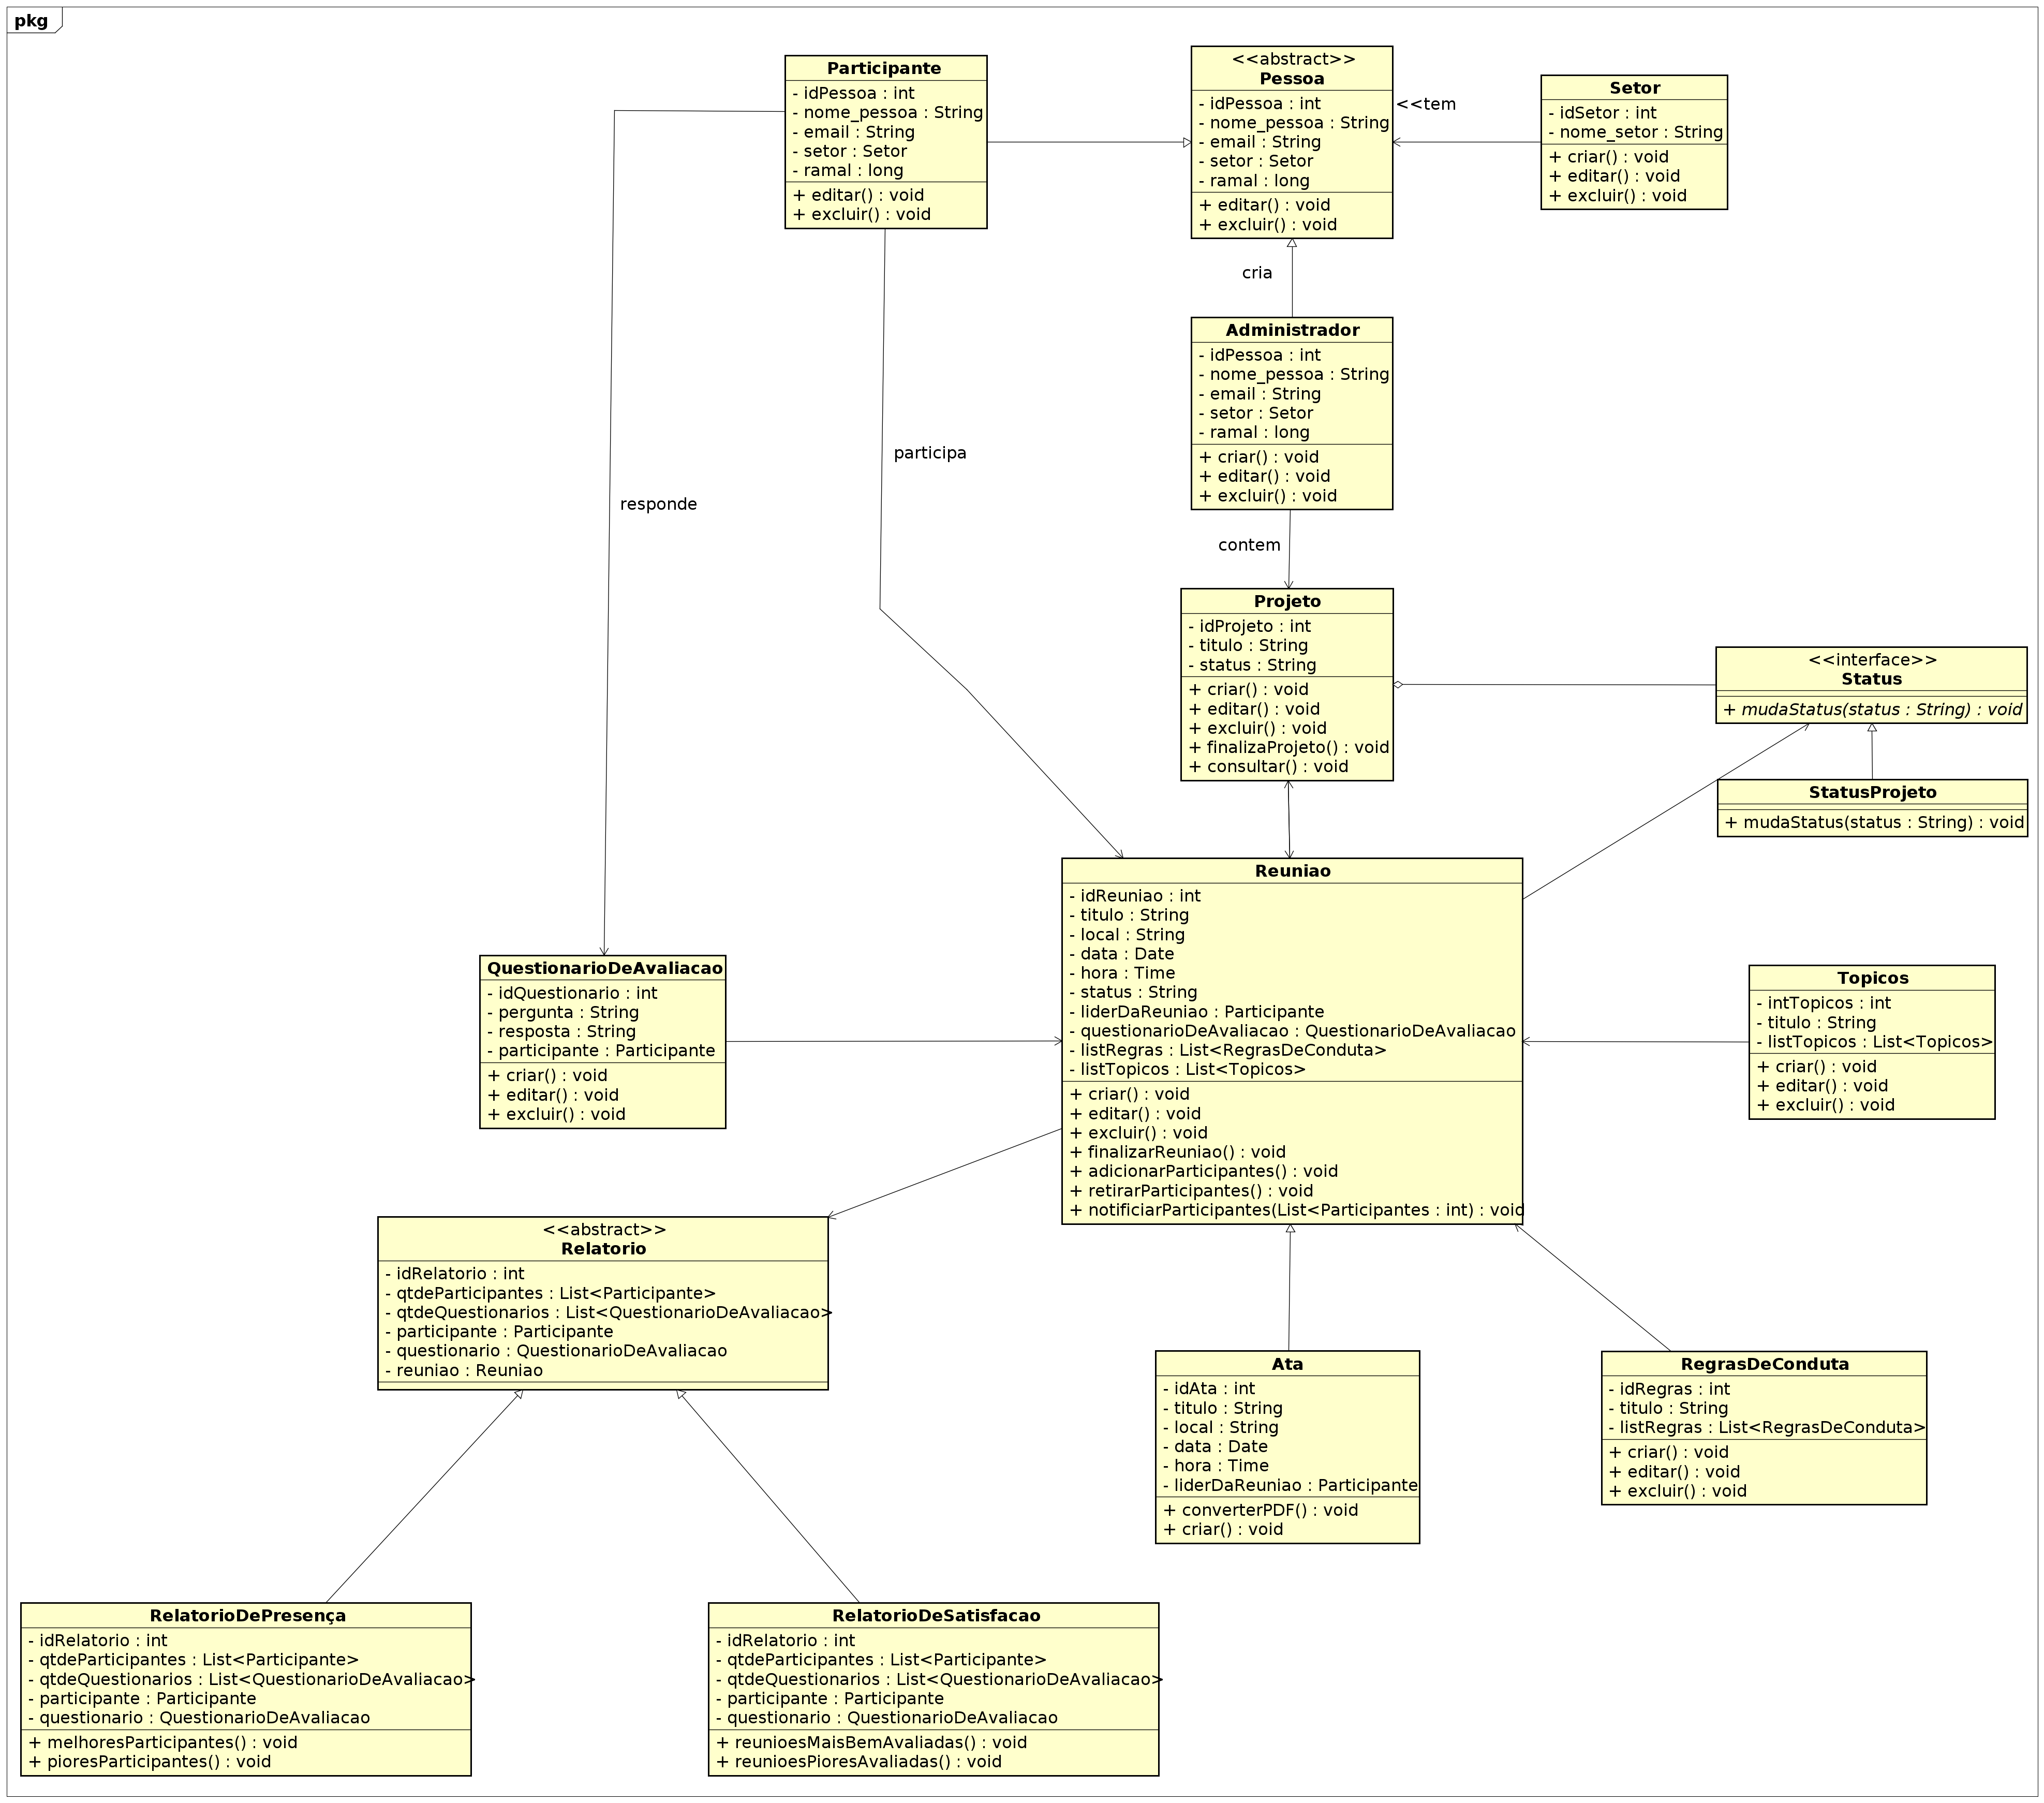
\includegraphics[width=1.0\textwidth]{figuras/diagramaDeClasse.png}
	\caption{Diagrama de Classe. Fonte: Própria}
	\label{img:diagrama_de_classe}
\end{figure}

\subsection{Banco de Dados}

\subsubsection{Modelo Conceitual}

\begin{figure}[H]
	\centering
	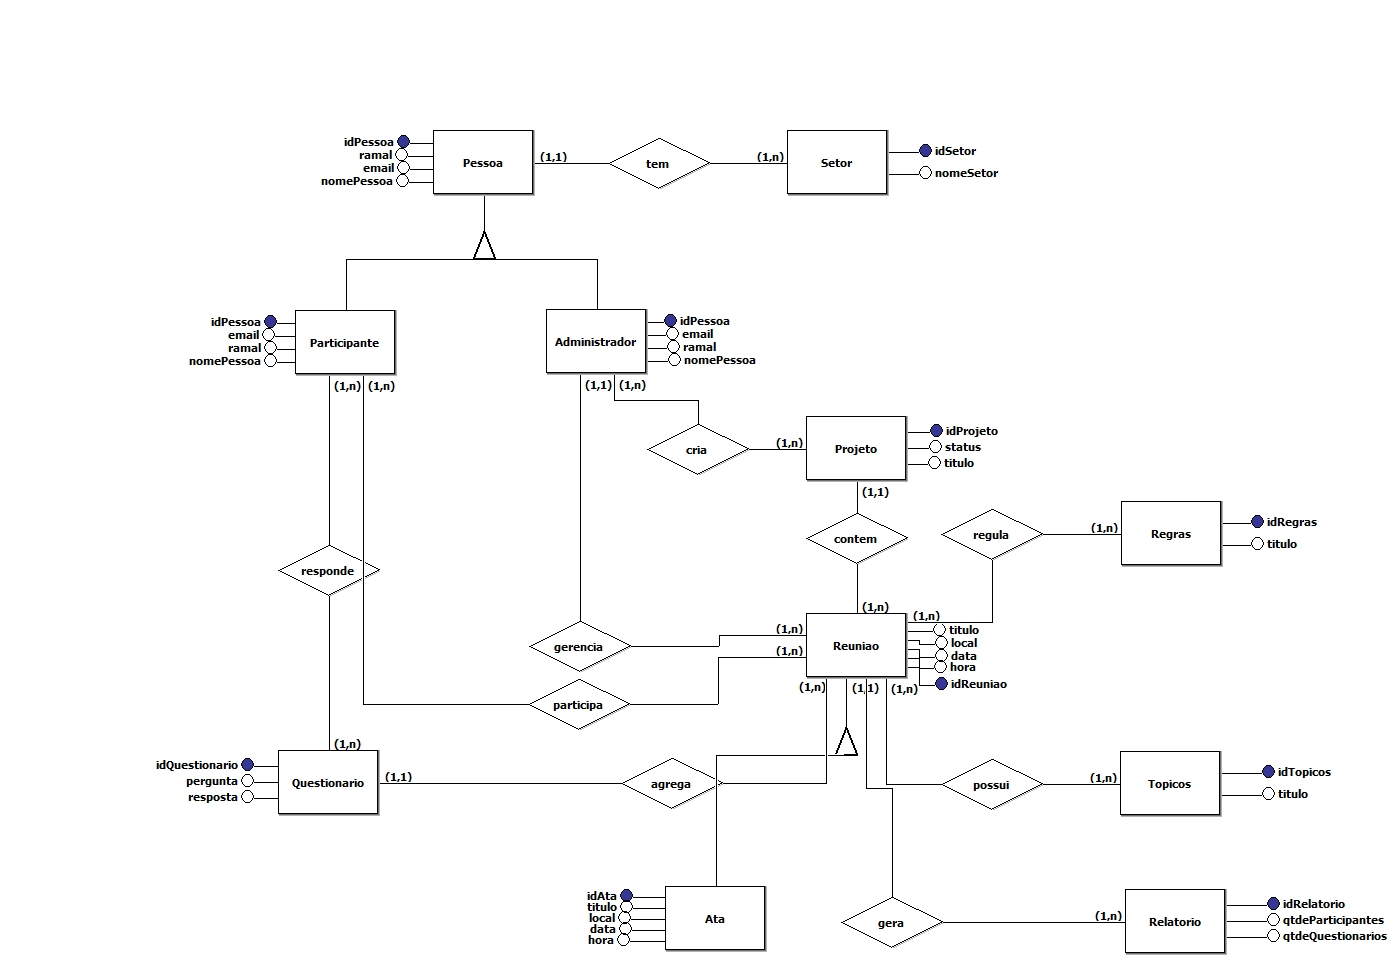
\includegraphics[width=1.0\textwidth]{figuras/bancoDeDados.jpg}
	\caption{Banco de Dados Modelo Conceitual. Fonte: Própria}
	\label{img:banco_conceitual}
\end{figure}

\subsubsection{Modelo Lógico}

\begin{figure}[H]
	\centering
	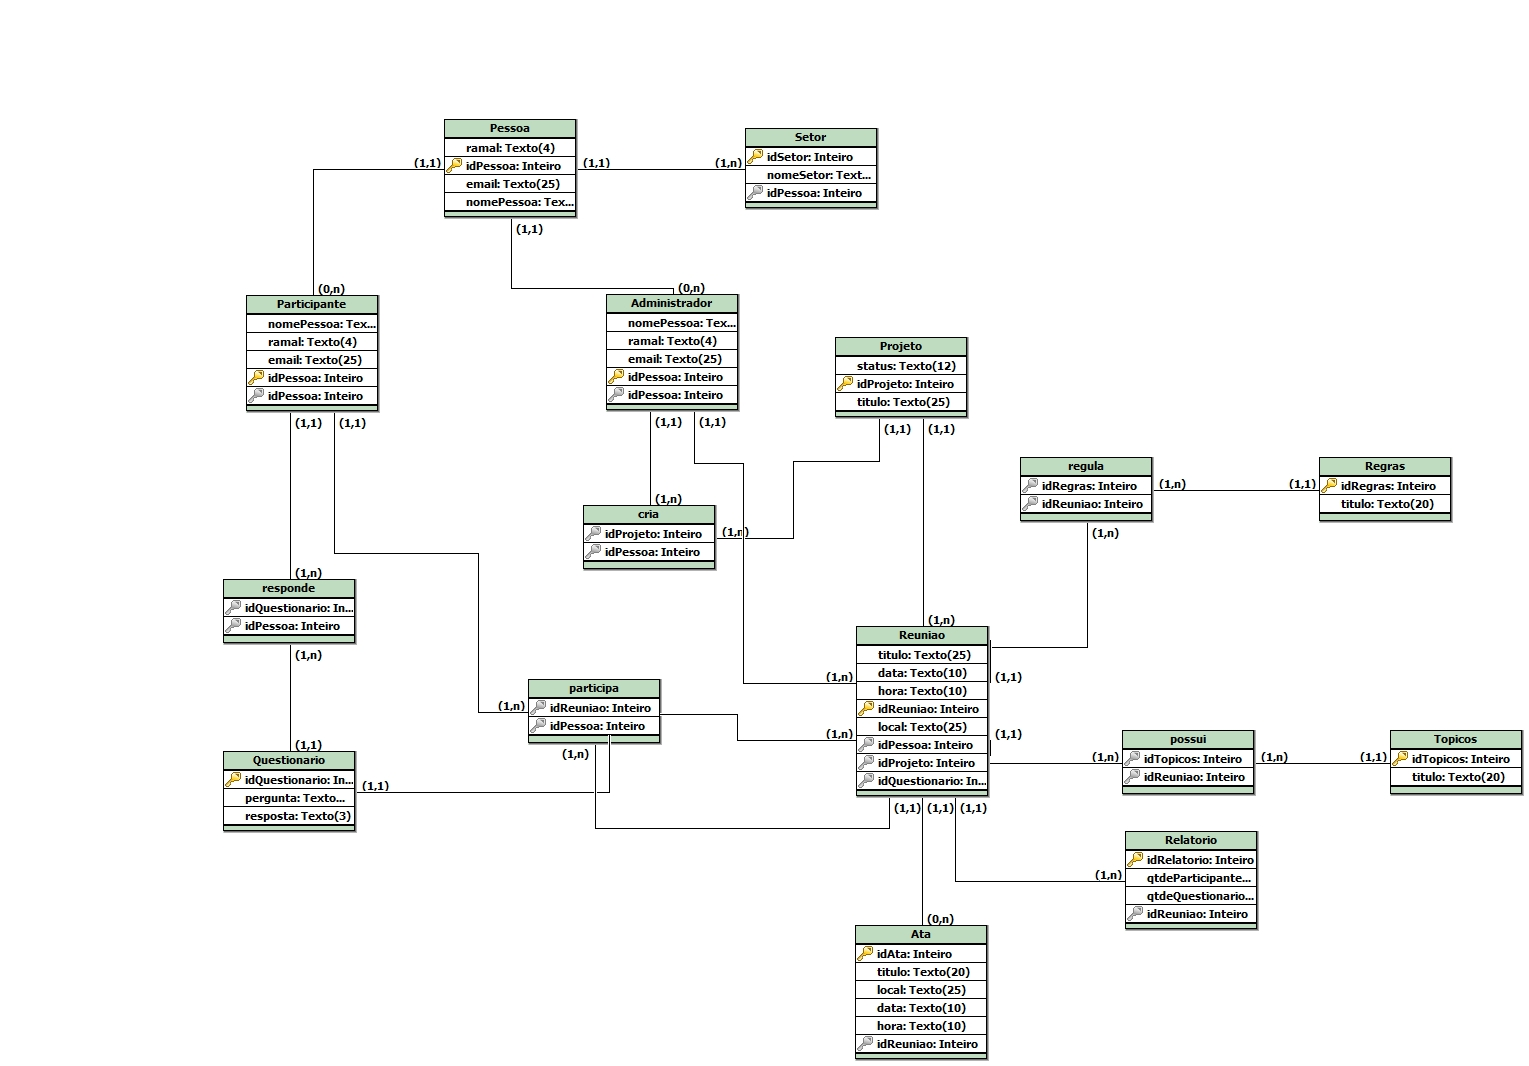
\includegraphics[width=1.0\textwidth]{figuras/bancoDeDadosLogico.jpg}
	\caption{Banco de Dados Modelo Lógico. Fonte: Própria}
	\label{img:banco_logico}
\end{figure}

\subsection{Front-End}

No tópico \ref{sec:front-end}, foi explicado e exemplificada algumas linguagens \textit{front-end}. A linguagem \textit{front-end} escolhida para este projeto, foi o \textit{React}, pois além de facilitar o desenvolvimento e interação com usuário final, é uma das mais utilizadas ao redor do mundo, então facilita uma manutenção futura e evolução do \textit{software}.

\subsection{Back-End}

No tópico \ref{sec:back-end}, foi explicado e exemplificado algumas linguagens \textit{back-end}. A linguagem \textit{back-end} escolhida para este projeto, foi a \textit{Python Django-Rest}, pois tem uma ótima conexão com a linguagem \textit{front-end}, e por ser muito utilizada, possibilitando assim uma manutenção e evolução futura.

\subsection{Protótipos}

Foram elaborados alguns protótipos para auxiliar o desenvolvimento deste projeto, sendo possível visualiza-los nos apêndices \ref{ch:prototipos}.

\subsection{Arquitetura do Projeto}

Neste projeto é feita uma adaptação ao padrão MVC, exemplificado no tópico \ref{sec:mvc}, por conta da escolha da linguagem \textit{front-end}. O \textit{React} possui um padrão arquitetural diferente do MVC, chamado de arquitetura de componentes. Esse padrão possui semelhanças ao MVC, e o que será utilizado dele será a parte da \textit{View}. Enquanto a linguagem \textit{back-end} é responsável por trabalhar os dados provindos do \textit{front-end} e oferecer um retorno a ele. 

A seguir será mostrado como funciona separadamente o \textit{React},relacionado ao \textit{front-end} que engloba a \textit{View}, enquanto o \textit{Python Django-Rest} é responsável pelo \textit{back-end} e que engloba a \textit{Model} e a \textit{Controller}:

\begin{figure}[H]
	\centering
	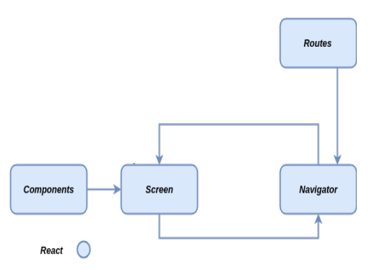
\includegraphics[width=1.0\textwidth]{figuras/diagrama_react.png}
	\caption{Diagrama React}
	\label{img:diagrama_react}
\end{figure}

\begin{figure}[H]
	\centering
	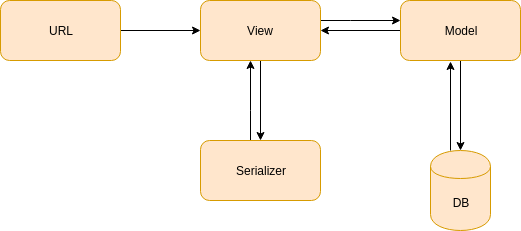
\includegraphics[width=1.0\textwidth]{figuras/django_rest.png}
	\caption{Diagrama Django REST Framework}
	\label{img:diagrama_rest}
\end{figure}

\section{Ferramentas Auxiliares}

Na Tabela \ref{tab:ferramentas_auxiliares} é mostrada as figuras que compõem este projeto.

\begin{table}[H]
	\begin{tabular}{|p{5.0cm}|p{10.0cm}|} 
	\hline
	\textbf{Ferramenta} & \textbf{Uso} \\ \hline
	\textbf{Astah UML} & Diagrama de Casos de Uso. \\ \hline
	& Diagrama de Classe \\ \hline
	\textbf{Bizagi Modeler} & Modelagem dos Processos \\ \hline
	\textbf{BrModelo} & Diagrama de Banco de Dados \\ \hline
	\textbf{Gantter} & Cronograma \\ \hline
	\end{tabular}
	 \caption{Ferramentas Auxiliares}
	 \label{tab:ferramentas_auxiliares}
\end{table}

\section{Cronograma TCC 2}

\begin{figure}[H]
	\centering
	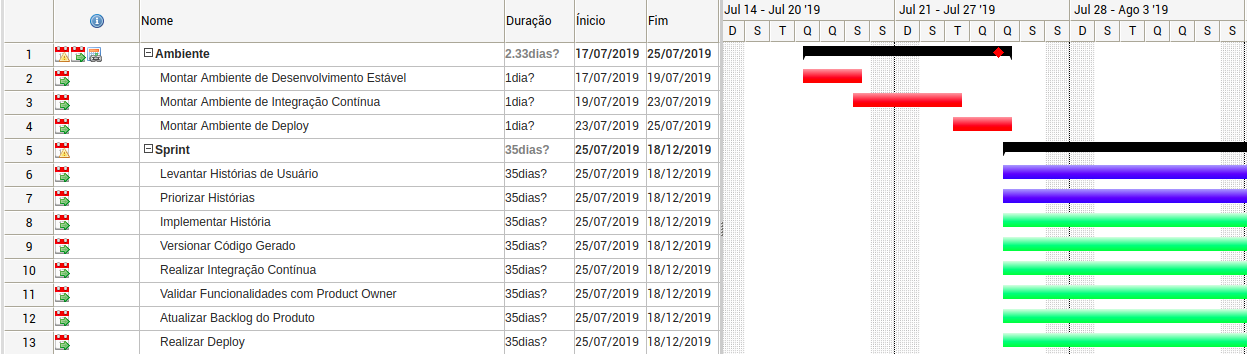
\includegraphics[width=1.1\textwidth]{figuras/cronograma.png}
	\caption{Cronograma TCC 2}
	\label{img:cronograma}
\end{figure}